%%%%%%%%%%%%%%%%%%%%%%%%%%%%%%%%%%%%%%%%%
% Dreuw & Deselaer's Poster
% LaTeX Template
% Version 1.0 (11/04/13)
%
% Created by:
% Philippe Dreuw and Thomas Deselaers
% http://www-i6.informatik.rwth-aachen.de/~dreuw/latexbeamerposter.php
%
% This template has been downloaded from:
% http://www.LaTeXTemplates.com
%
% License:
% CC BY-NC-SA 3.0 (http://creativecommons.org/licenses/by-nc-sa/3.0/)
%
%%%%%%%%%%%%%%%%%%%%%%%%%%%%%%%%%%%%%%%%%

%----------------------------------------------------------------------------------------
%	PACKAGES AND OTHER DOCUMENT CONFIGURATIONS
%----------------------------------------------------------------------------------------

\documentclass[final,hyperref={pdfpagelabels=false}]{beamer}

\usepackage[orientation=portrait,size=a1,scale=1.3]{beamerposter} % Use the beamerposter package for laying out the poster with a portrait orientation and an a0 paper size

\usetheme{I6pd2} % Use the I6pd2 theme supplied with this template

\usepackage[english]{babel} % English language/hyphenation

\usepackage{amsmath,amsthm,amssymb,latexsym} % For including math equations, theorems, symbols, etc

%\usepackage{times}\usefonttheme{professionalfonts}  % Uncomment to use Times as the main font
%\usefonttheme[onlymath]{serif} % Uncomment to use a Serif font within math environments

\boldmath % Use bold for everything within the math environment

\usepackage{booktabs} % Top and bottom rules for tables

\graphicspath{{figures/}} % Location of the graphics files

\usecaptiontemplate{\small\structure{\insertcaptionname~\insertcaptionnumber: }\insertcaption} % A fix for figure numbering

%----------------------------------------------------------------------------------------
%	TITLE SECTION 
%----------------------------------------------------------------------------------------

\title{\huge A Sphere Model for Atrial Fibrillation} % Poster title

\author{Tigany Zarrouk \& Mattia Gaggi } % Author(s)

\institute{Supervisor: Kim Christensen.  Condensed Matter Theory Group---Imperial College London} % Institution(s)

%----------------------------------------------------------------------------------------
%	FOOTER TEXT
%----------------------------------------------------------------------------------------

\newcommand{\leftfoot}{} % Left footer text

\newcommand{\rightfoot}{} % Right footer text


%----------------------------------------------------------------------------------------

\begin{document}

\addtobeamertemplate{block end}{}{\vspace*{2ex}} % White space under blocks

\begin{frame}[t] % The whole poster is enclosed in one beamer frame

\begin{columns}[t] % The whole poster consists of two major columns, each of which can be subdivided further with another \begin{columns} block - the [t] argument aligns each column's content to the top

\begin{column}{.02\textwidth}\end{column} % Empty spacer column

\begin{column}{.465\textwidth} % The first column

%----------------------------------------------------------------------------------------
%	OBJECTIVES
%----------------------------------------------------------------------------------------

\begin{block}{Objectives}

\begin{enumerate}
\item Replicate original model of Atrial Fibrillation (AF) from Christensen \emph{et al.}
\item Incorporate restitution of heart cells into the model. 
\item Model on more realistic morphology via translating model onto a sphere and adding restitution. 
\item Analyse to see if there is enhanced risk with the new model, using new morphology and model basis, to create a more accurate AF model.
\end{enumerate}

\end{block}

%----------------------------------------------------------------------------------------
%	INTRODUCTION
%----------------------------------------------------------------------------------------
            
\begin{block}{Introduction}

\begin{itemize}
\item Atrial Fibrillation (AF) is a type of cardiac arrhythmia and one of the major causes of stroke and heart failure. AF is also the most widespread cardiac condition, with over 30 millions of people worldwide suffering from it. In the UK, expenses related to this disease account for more than $1\%$ of the total budget of the National Health Service, which is more than $800$ million pounds. Atrial fibrillation usually manifests itself in patients affected through alterations of the normal cardiac rhythm lasting short periods of time (also called fibrillation episodes).\\
\end{itemize}


\end{block}


\begin{block}{Phenomenology of Atrial Fibrillation}


	\begin{itemize}
	\item Each heart beat originates as an electric signal in the sinoatrial (SA) node that propagates first into the atria, then through the atrioventricular (AV) node, through Purkinje fibres 		and finally from the ventricular endocardium to the ventricular epicardium. The electric signal is conducted in the cardiac muscle cells thanks to the polarisation mechanism of the cell 		membrane. 


	\item When the electric impulse propagates a single muscle cell goes through three stages:

		\begin{itemize}
 		 \item \textit{Excitable state}: the muscle cell is at rest with a negative built up potential.
  										
  		\item \textit{Excited state}: the muscle cell is excited by its excited neighbours and the Voltage of the cell is at its peak. 
  		\item \textit{Refractory state} :the muscle cell goes through a phase during which it can't be excited again - this period is called \textit{refractory period)}.
		\end{itemize}  

	\item Where the refractory period depends on the last time a cell was excited and is always fixed to a constant.\\



	\item AF is correlated to the amount of \textbf{ fibrosis} in the cardiac tissue which generates a process called reentry. \\
	During reentry the electric signal wavefront propagation breaks. It has been shown a clear link between fibrosis and AF
	Even though many treatments have been developed, the mechanisms behind this condition are not completely understood and AF remains a major topic in medical research. \\
	The current research revolves around three possible approaches:
	\end{itemize}

%\begin{frame}
%\smartdiagram[bubble diagram]{Current research,
 %Physiological \\ models, Image-Based \\ Models, \textbf{ CA Models}, antiarrhythmic \\ drugs) }
% \end{frame}
 Our research is based on expanding on the work done by Kim Christensen on CA (Cellular Automata) models \cite{Christensen}.


\end{block}

\begin{block}{Results: Connectome}

%\centering
\begin{figure}
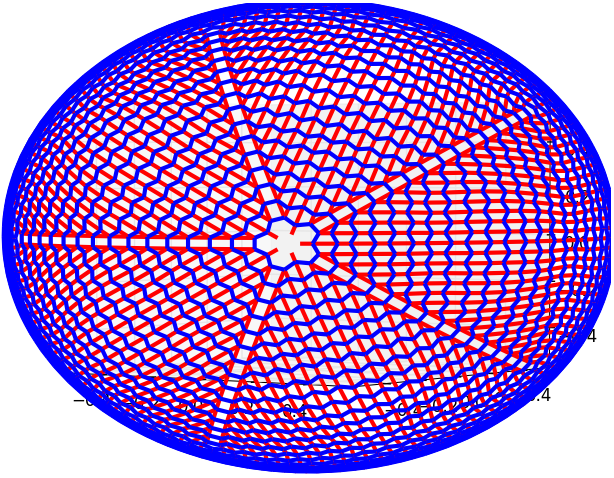
\includegraphics[width=0.7\linewidth]{connectome}
\caption{Hemisphere of possible connections defined on the sphere model. Each vertex corresponds to a face. Longitudinal connections are in red, transversal are in blue. Starts from a single pentagon on the icosphere and then can be seen to propagate outwards. }
\end{figure}

\end{block}


%\end{column}

%----------------------------------------------------------------------------------------

\end{column} % End of the first column

\begin{column}{.03\textwidth}\end{column} % Empty spacer column
 
\begin{column}{.465\textwidth} % The second column

%----------------------------------------------------------------------------------------
%	RESULTS
%----------------------------------------------------------------------------------------

%------------------------------------------------

\begin{block}{Results: Sphere and Previous model}

%\centering
\begin{figure}
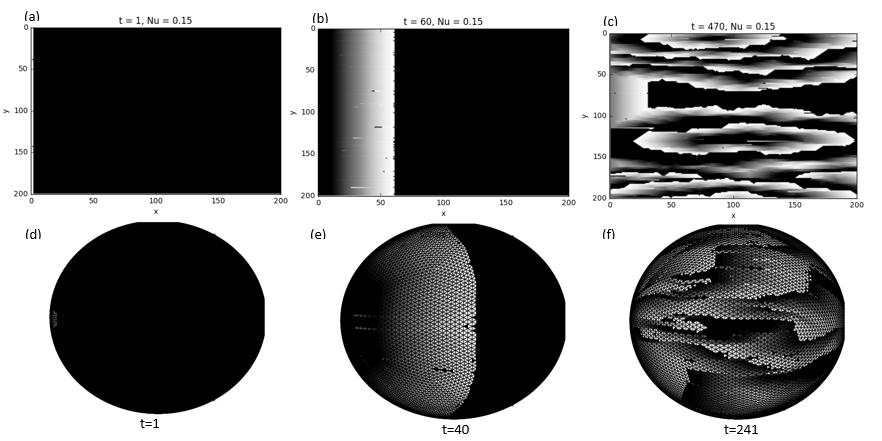
\includegraphics[width=0.8\linewidth]{combchristensenspherefib}
\caption{Figures of: Christensen \emph{et al.}'s model at times of t=1, t=60 and t=470,for a, b and c, respectively, and the sphere model at times of t=1, t=41 and t=241 for d, e and f respectively. Normal wavefront propagation seen starting from pentagonal node in the leftmost figures.In figure e, the excitation wavefront propagates around the sphere, mimicking Christensen \emph{et al.}'s model, b. On the right, chaotic, fibrillatory activity has arisen from reentry circuit spontaneously manifesting itself in c and f.}
\end{figure}

\end{block}


\begin{block}{Implementing Restitution }

In Christensen \emph{et al.}'s model, the refractory period of each muscle cell was always fixed, this is not what happens in a real heart.
In a real heart the refractory period depends on the heart beat rate and on the last time each cell it was excited. The relationship between refractory period and heart beat rate is called restitution.
\end{block}



\begin{block}{Model on a Sphere}


\begin{itemize}
\item In research by Fedotov, a cellular automaton model was constructed on the surface of a triangulated sphere to model spiral rotor waves on a closed, heterogeneous surface \cite{Fedotov}. It was shown that both a decrease in refractory period and conduction velocity from a "healthy" myocardium state, where no irregular excitation waves above 300bpm are observed, resulted in an area where spiral waves were formed. In addition, a multi-electrode system was created to study the localization of AF sources by simulated electrograms. 
\end{itemize}

\end{block}
%------------------------------------------------

\begin{block}{Results: Figure}

%\centering
\begin{figure}
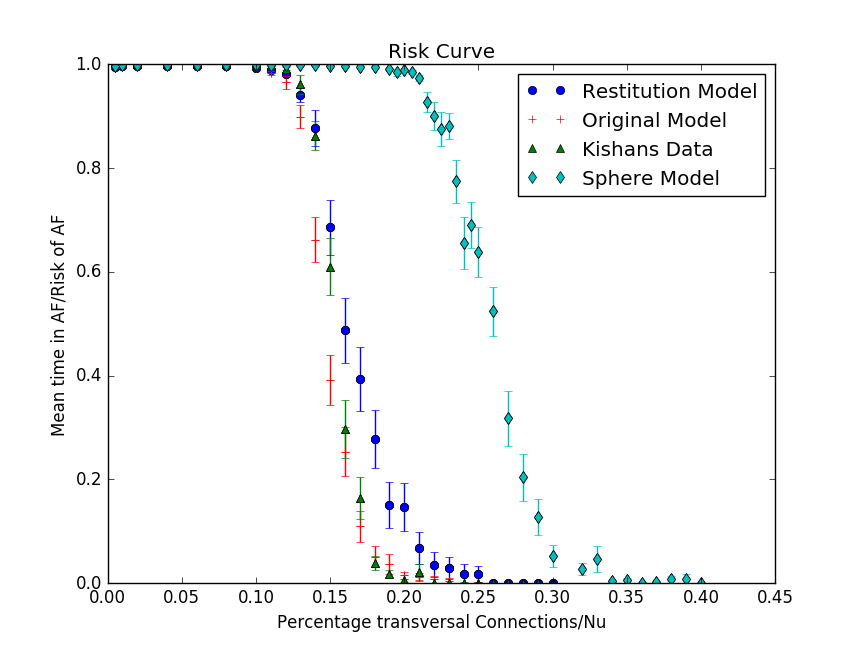
\includegraphics[width=0.65\linewidth]{xriskcurvesphere}
\caption{Figure of the Risk Curve of all the systems analysed. Y-axis: probablility of a realisation being in AF, x-axis: value of $\nu$, the  probability of a transversal connection between cells}
\end{figure}

\end{block}

%----------------------------------------------------------------------------------------
%	CONCLUSION
%----------------------------------------------------------------------------------------

\begin{block}{Conclusion}
\begin{itemize}
\item A simplified mechanism of AF had been achieved by Christensen \emph{et al.'s} model through the modelling of heart muscle fibre connectivity while incorporating the effects of fibrosis. This model was improved upon by the additon of the restitution process, making AF more risky. By translating the model to a sphere, the steady growth of heart muscle fibres from the sino-atrial node could be replicated, while simulating a more realisitc morphology of the atria. The risk of AF was seen to be higher, than with the original model. Verification of this model can be achieved with the analysis of the proportion of fibrosis in atrial heart tissue. 
\end{itemize}
\end{block}

%----------------------------------------------------------------------------------------
%	REFERENCES
%----------------------------------------------------------------------------------------

\begin{block}{References}
        
\nocite{*} % Insert publications even if they are not cited in the poster
\small{\bibliographystyle{unsrt}
\bibliography{sample1}}

\end{block}



%----------------------------------------------------------------------------------------
%	CONTACT INFORMATION
%----------------------------------------------------------------------------------------

%\setbeamercolor{block title}{fg=black,bg=orange!70} % Change the block title color

%\begin{block}{Contact Information}

%\begin{itemize}
%\item Web: \href{http://www.university.edu/smithlab}{http://www.university.edu/smithlab}
%\item Email: \href{mailto:john@smith.com}{john@smith.com}
%\item Phone: +1 (000) 111 1111
%\end{itemize}

%\end{block}

%----------------------------------------------------------------------------------------

\end{column} % End of the second column

\begin{column}{.015\textwidth}\end{column} % Empty spacer column

\end{columns} % End of all the columns in the poster

\end{frame} % End of the enclosing frame

\end{document}